\documentclass[11pt, oneside]{article}   	% use "amsart" instead of "article" for AMSLaTeX format
\usepackage{geometry}                		% See geometry.pdf to learn the layout options. There are lots.
\geometry{letterpaper}                   		% ... or a4paper or a5paper or ... 
%\geometry{landscape}                		% Activate for rotated page geometry
%\usepackage[parfill]{parskip}    		% Activate to begin paragraphs with an empty line rather than an indent
\usepackage{graphicx}				% Use pdf, png, jpg, or eps§ with pdflatex; use eps in DVI mode
								% TeX will automatically convert eps --> pdf in pdflatex		
\usepackage{amssymb}

\usepackage{listings}

\usepackage[T1]{fontenc}
\usepackage[polish]{babel}
\usepackage[utf8]{inputenc}
\usepackage{lmodern}
\selectlanguage{polish}


\lstset{language=Matlab} 

%SetFonts

%SetFonts

\title{MNUM-PROJEKT, zadanie 3.17}
\author{Marcin Dziedzic}
%\date{}							% Activate to display a given date or no date

\begin{document}
\maketitle{}
\tableofcontents
\section{Zadanie I}
\subsection{Treść zadania}
Proszę znaleźć wszystkie zera funkcji
\begin{center}
$f(x) = 0.7xcos(x)-ln(x+1)$
\end{center}
w przedziale $[2,11]$, używając dla każdego zera programu z implementacją:\\
a) metody bisekcji\\
b) metody siecznych\\
c) metody Newtona\\

\subsection{Wyznaczanie miejsc zerowych funkcji}
Izolowanie pierwiastka Aby znalezc miejsce zerowe funkcji, trzeba po pierwsze
znalezc przedział, w kktórym ten pierwiastek na pewno sie znajduje. Jezeli
mamy dwa punkty a i b, to warunkiem wystarczajacym istnienia pierwiastka
jest zaleznosc:
\begin{center}
	$f(a)f(b)<0$
\end{center}
Oczywiscie tych miejsc zerowych moze byc wiecej w tym przedziale w dodatku
gdy f(a)f(b)>0 to wcale nie znaczy, ze pierwiastka w tym przedziale nie ma.
Warto zatem posłuzyc sie wykresem funkcji i odizolowac pierwiastki czyli okreslic
przedziały, w których miejsca zerowe sie znajduja, gdyz znakomita wiekszosc
metod iteracyjnych ich wyznaczania wymaga własnie odizolowania pierwiastka.
Aby znalezc wszystkie przedziały, w którym znajduja sie pierwiastki napisałem
funkcje, która zwraca macierz przdziałów, w których znajduja sie zera funkcji.
Ponizej przedstawiam implementacje wraz z komentarzem.
\begin{lstlisting}[caption=Implementacja RootIsolation]
% funkcja znajduje przedzialy, w ktorych znajduja 
% sie zeram funkcji. Przyjmuje 3 argumenty:
% fun - funkcja, w ktorej chcemy odizolowac pierwiastki
% <a,b> - przedzial.
% zwraca macierz przedzialow w ktorych znajduja sie 
% pierwiastki
function y = RootIsolation(fun,a,b)
  isroot=false;
  n=1;% ilosc przedzialow z pierwiastkiami 
  d=0.5;% dlogosc poczatkowa przedzialu
  while a+d<=b% dopoki petla nie przejdzie 
% po calym zadanym przedziale
    if feval(fun,a)*feval(fun,a+d)<=0
% jesli w przedziale jest pierwiastek
      isroot=true;
      y(n,1)=a;
      y(n,2)=a+d;% na pierwszej kolumnie zapisujemy 
% punkt poczatkowy, na drugiej koncowy
      n++;% zwiekszamy rozmiar macierzy
      a=a+d;% zaczynamy od miejsca gdzie konczyl 
% sie poprzeni przedzial
      d=0.25;% d znowu na 0.05 ponizej juz bedzie 0.05
    end
    d*=2;
  end
  if isroot==false% gdy brak pierwiastkow zwroc 0
    y=0;
  end
end

	
\end{lstlisting}



\subsection{Metoda bisekcji}
\subsubsection{Opis teoretyczny}
Teoretyczny zarys metody bisekcji możemy przybliżyć poniższym algorytmem:
\begin{enumerate}
  \item Począwszy od przedziału startowego $[a,b]$ = $[a_{0},b_{0}]$ obliczamy środek przedziału $c_{n}$,
  	$c_{n} = \frac{a_{n}+b_{n}}{2}$
  i obliczamy wartość $f(x)$ w tym punkcie. 
  \item Obliczamy iloczyny $f(a_{n})*f(c_{n})$ oraz $f(b_{n})*f(c_{n})$ i jako nowy przedział $[a_{n=1},b_{n+1}]$
  wybieramy argumenty tego iloczynu którego wartość jest ujemna. 
\end{enumerate} 
Kroki te powtarzamy aż do momentu uzyskania $f(c_{n})<\delta$ gdzie $\delta$ to oczekiwana dokładność rozwiązania. W przypadku "płaskich"  funkcji warto też kontrolować długość rozpatrywanego przedziału. 
Dokładność wyniku zależy jedynie od ilości iteracji dlatego metoda jest zbieżna liniowo z ilorazem zbieżności 0.5, co czyni ją stosunkowo wolno zbieżną w przypadku wyboru szerokiego przedziału początkowego. 


\subsubsection{Realizacja w programie Matlab}
\begin{lstlisting}[caption=Implementacja metody bisekcji]
% Funkcja wyznaczajaca punkty zerowe funkcji metoda bisekcji
%
% IN:
% a0, b0 - zakres
% fun - funkcja 
% iter - maksymalna liczba iteracji
%
% OUT:
% solution - wyznaczone miejsce zerowe

function soluiton = md_bisection(fun,a0,b0,iter)

  a = a0; 
  b = b0;
  % inicjalizacja wartosciami poczatkowymi
  fa =feval(fun,a);     
  fb =feval(fun,b);
  for k=1:iter
    % obliczenie srodka odcinka
    xm = a + 0.5*(b-a);    
    %  f(xm) 
    fm = feval(fun,xm);      
    fprintf('%3d    [%12.10f;%12.10f]	%12.16f     %12.3e\n',k,a,b,xm,fm);
    if(fm == 0)
        return
    end
    %  Zero lezy w przedziale [xm,b], zamiana a
    if sign(fm)==sign(fa)    
        a = xm;
        fa = fm;
    %  Zero lezy w przedziale [a,xm], zamiana b
    else                     
        b = xm;
        fb = fm;
    end
    %dodatkowy warunek zakonczenia wykonywania
    if(fm == 0) 
        return
    end
  end
  soluiton = xm; 
  return
end
	

		
\end{lstlisting}


\subsection{Metoda siecznych}
Metoda siecznch jest bardzo podobna do metody bisekcji, różni się tym, iż przez krańce aktualnego przedziału prowadzimy prostą, która przecina oś rzędnych w punkcie \begin{large}
$x_{0}$
\end{large}. Następnie prowadzimy kolejną prostą przez punkt \begin{large}
$f(x_{n})$ 
\end{large} i poprzedni punkt \begin{large}
$f(x_{n-1})$ 
\end{large}. Warto zaznaczyć, że nie dbamy tutaj o przedział izolacji pierwiastka, ani nawet o znak iloczynu wartości na krańcach aktualnego przedziału.\\\\
Wzór na n+1 punkt, przez który ma przejść prosta:
\begin{large}
$x_{n+1}=\frac{x_{n-1}f(x_{n})-x_{n}f(x_{n-1})}{f(x_{n})-f(x_{n-1})}$
\end{large}

Rząd zbieżności metody siecznych wynosi \begin{large}$\frac{1+\sqrt{5}}{2}$\end{large} zatem metoda ta jest szybsza od metody bisekcji, lecz w praktyce może okazać się niezbieżna kiedy przedział izolacji nie jest dostatecznie mały, gdyż jest ona zbieżna tylko lokalnie, a nie globalnie jak poprzednia metoda. 
\subsubsection{Realizacja w programie Matlab}
\begin{lstlisting}[caption=Implementacja metody siecznych]
% Funkcja wyznaczajaca punkty zerowe funkcji metoda siecznych
%
% IN:
% a0, b0 - zakres
% fun - funkcja 
% iter - maksymalna liczba iteracji
%
% OUT:
% solution - wyznaczone miejsce zerowe
function solution = md_secans(fun, a0, b0, iter)
  a = a0;
  b = b0;
  % poczatkowa wartosc funkcji
  fa = feval(fun,a); 
  for k = 1:iter
    fb = feval(fun,b);
    dx = fb * (b-a) / (fb-fa); 
    xm = b-dx; 
    if(isnan(xm))
        return
    end
    a = b;
    b = xm;
    fa = fb;
    solution = b;
    fprintf('%3d	[%12.10f;%12.10f]   %12.16f     %12.3e\n',k,a,b,xm,fb);
    %dodatkowy warunek zakonczenia wykonywania
    if(fb == 0) 
        return
    end
  end
end
\end{lstlisting}

\subsection{Metoda Newtona}
\subsubsection{Opis teoretyczny}
Metoda Newtona polega na wyznaczeniu częściowego (uciętego) rozwinięcia w szereg Taylora danej funkcji, które możemy traktować jak liniowe przybliżenie funkcji według wzoru:\
  	\begin{center}
  	$f(x) \approx f(x_{n})+f'(x_{n})(x-x_{n})$
	\end{center}
Następnie wyznaczamy kolejne punkty iteracji poprzez przyrównanie do zera otrzymanej aproksymacji:\\
\begin{center}
$f(x_{n})+f'(x_{n})(x_{n+1}-x_{n}) = 0$
\end{center}
Prowadzi to do zależności iteracyjnej danej następującym wzorem:\\
\begin{center}
$x_{n+1} = x_{n}-\frac{f(x_{n})}{f'(x_{n})}$
\end{center}
Metoda Newtona jest zbieżna jedynie lokalnie, ponieważ wyznaczając styczną do wykresu w danym punkcie możemy w przypadku ujemnego znaku pochodnej dojsć do rozbieżności. Dla przypadków pochodnej większej od zera metoda jest zbieżna kwadratowo. Rząd zbieżności wynosi 2.

\subsubsection{Realizacja w programie Matlab}
\begin{lstlisting}[caption=Implementacja metody Newtona]

% Funkcja wyznaczajaca punkty zerowe funkcji metoda Newtona
%
% IN:
% a0 - lewa strona zakresu
% fun - funkcja 
% iter - maksymalna liczba iteracji
%
% OUT:
% solution - wyznaczone miejsce zerowe
function solution = md_newton(fun, a0,iter)
  x0 = a0; 
  for k = 1:iter
    [fold, fpold] = feval(fun,x0); 
    dx = fold / fpold; 
    x0 = x0 - dx;
    fprintf('%3d	%12.10f     %12.16f     %12.3e \n',k,dx,x0,fold);
    if(fold == 0)
        return
    end
    %dodatkowy warunek zatrzumania
	if fold==0 
        solution = x0;
        break; 
    end
  end
end

\end{lstlisting}


\subsection{Analiza danych wejściowych}
W celu wyznaczenia przedziałów izolacji miejsc zerowych został wykorzystany algorytm opisany w skrypcie prof. Tatjewskiego. Wstępna analiza danych rozpoczyna się od wygenerowania wykresu funkcji w danym przedziale i na tej podstawie wyboru przedziału startowego dla algorytmu. Następnie w podanym przedziale w pętli badany jest znak iloczynu funkcji w punktach granicznych. Jeżeli jest on ujemny, oznacza to występowanie miejsca zerowego w danym przedziale. Jeżeli nie, to przedział jest rozszerzany do momentu przekroczenia przedziału danego w zadaniu. 
Poniżej wykres funkcji z zaznaczonymi przedziałami izolacji wyznaczonymi przez algorytm. 

\begin{figure}[h]
%\caption{Wykres z zaznaczonymi przedziałami startowymi}
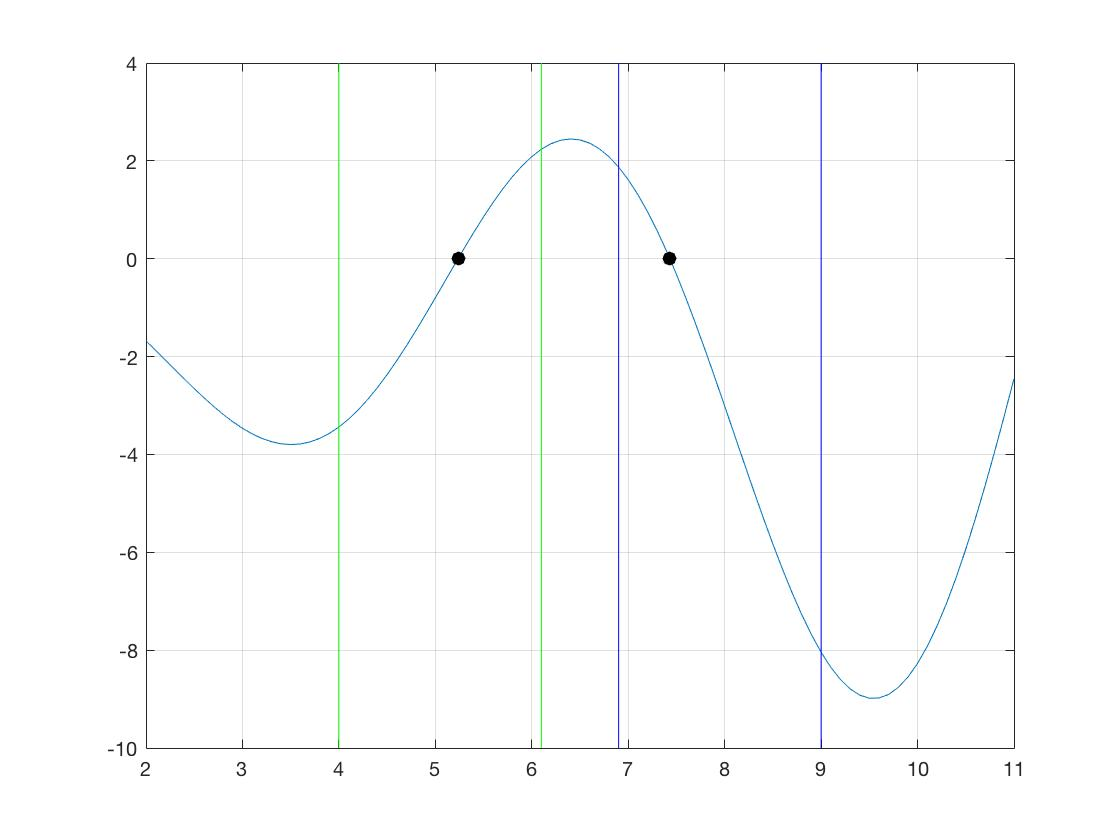
\includegraphics[width=\textwidth]{figure1.jpg}
\end{figure}

\subsubsection{Realizacja w programie Matlab}
\begin{lstlisting}[caption=Skrypt rozwiązujący zadanie nr 1]

% zadanie nr 1

clear; 
x  = 2 : 0.1 : 11;
plot(x, md_fun_1(x))
grid on
axis([2 11 -10 4])
hold on
plot([4 4], [-10 4], 'g-');
plot([6.1 6.1], [-10 4], 'g-');
plot([6.9 6.9], [-10 4], 'b-');
plot([9 9], [-10 4], 'b-');
plot(5.2353163129141116, 0, '.','MarkerSize', 24, 'MarkerEdge', 'k');
plot(7.4317177653721664, 0,'.','MarkerSize',24,'MarkerEdge','k');

n=100; 
x1 = 4; 
x2 = 5; 

% algorytmiczne wyznaczanie przedzialow izolacji
for k=1:2
    for j=1:n
        if md_fun_1(x1)*md_fun_1(x2)<0
            a = x1;
            b = x2;
            fprintf('Wyniki dla %d miejsca zerowego w przedziale [%d,%d]\n',k,a,b);
            bisection('md_fun_1',a,b,100);
            secant('md_fun_1',a,b,100);
            newton('md_fun_1',a,100);
            x1 = 8; 
            x2 = 9; 
            break;
        elseif abs(md_fun_1(x1))<abs(md_fun_1(x2))
            x1 = x1+1.1*(x1-x2);
        else
            x2 = x2+1.1*(x2-x1);
        end
        %wyjscie z petli po przekroczeniu przedzialu
        if(x1>11)&&(x2<(2))
            break; 
        end
    end
end

\end{lstlisting}

\begin{center}
\begin{tabular}{ c c c }
 cell1 & cell2 & cell3 \\ 
 cell4 & cell5 & cell6 \\  
 cell7 & cell8 & cell9    
\end{tabular}
\end{center}

\subsection{Rozwiązanie}
\subsubsection{Metoda bisekcji}

\begin{center}
\begin{tabular}{ |c|c|c|c| } 
\hline
\multicolumn{4}{|c|}{Pierwsze miejsce zerowe} \\
 \hline
 nr & przedzial & rozwiazanie & wartość \\
 \hline
1 & [4.0000000000;6.1000000000] & 5.0499999999999998 &   -6.291e-01 \\ 
  2 & [5.0500000000;6.1000000000] & 5.5749999999999993 &    1.081e+00 \\ 
  3 & [5.0500000000;5.5750000000] & 5.3125000000000000 &    2.576e-01 \\ 
  4 & [5.0500000000;5.3125000000] & 5.1812500000000004 &   -1.826e-01 \\ 
  5 & [5.1812500000;5.3125000000] & 5.2468750000000002 &    3.884e-02 \\ 
  6 & [5.1812500000;5.2468750000] & 5.2140625000000007 &   -7.163e-02 \\ 
  7 & [5.2140625000;5.2468750000] & 5.2304687500000000 &   -1.631e-02 \\ 
  8 & [5.2304687500;5.2468750000] & 5.2386718749999996 &    1.129e-02 \\ 
  9 & [5.2304687500;5.2386718750] & 5.2345703124999998 &   -2.510e-03 \\ 
 10 & [5.2345703125;5.2386718750] & 5.2366210937499993 &    4.389e-03 \\ 
 11 & [5.2345703125;5.2366210937] & 5.2355957031250000 &    9.399e-04 \\ 
 12 & [5.2345703125;5.2355957031] & 5.2350830078125004 &   -7.849e-04 \\ 
 13 & [5.2350830078;5.2355957031] & 5.2353393554687502 &    7.752e-05 \\ 
 14 & [5.2350830078;5.2353393555] & 5.2352111816406257 &   -3.537e-04 \\ 
 15 & [5.2352111816;5.2353393555] & 5.2352752685546875 &   -1.381e-04 \\ 
 16 & [5.2352752686;5.2353393555] & 5.2353073120117184 &   -3.028e-05 \\ 
 17 & [5.2353073120;5.2353393555] & 5.2353233337402347 &    2.362e-05 \\ 
 18 & [5.2353073120;5.2353233337] & 5.2353153228759766 &   -3.331e-06 \\ 
 19 & [5.2353153229;5.2353233337] & 5.2353193283081056 &    1.014e-05 \\ 
 20 & [5.2353153229;5.2353193283] & 5.2353173255920407 &    3.407e-06 \\ 
 21 & [5.2353153229;5.2353173256] & 5.2353163242340086 &    3.808e-08 \\ 
 22 & [5.2353153229;5.2353163242] & 5.2353158235549930 &   -1.646e-06 \\ 
 23 & [5.2353158236;5.2353163242] & 5.2353160738945004 &   -8.041e-07 \\ 
 24 & [5.2353160739;5.2353163242] & 5.2353161990642541 &   -3.830e-07 \\ 
 25 & [5.2353161991;5.2353163242] & 5.2353162616491318 &   -1.725e-07 \\ 
 26 & [5.2353162616;5.2353163242] & 5.2353162929415706 &   -6.719e-08 \\ 
 27 & [5.2353162929;5.2353163242] & 5.2353163085877892 &   -1.455e-08 \\ 
 28 & [5.2353163086;5.2353163242] & 5.2353163164108985 &    1.176e-08 \\ 
 29 & [5.2353163086;5.2353163164] & 5.2353163124993438 &   -1.395e-09 \\ 
 30 & [5.2353163125;5.2353163164] & 5.2353163144551207 &    5.184e-09 \\ 
 31 & [5.2353163125;5.2353163145] & 5.2353163134772327 &    1.894e-09 \\ 
 32 & [5.2353163125;5.2353163135] & 5.2353163129882887 &    2.495e-10 \\ 
 33 & [5.2353163125;5.2353163130] & 5.2353163127438158 &   -5.729e-10 \\ 
 34 & [5.2353163127;5.2353163130] & 5.2353163128660523 &   -1.617e-10 \\ 
 35 & [5.2353163129;5.2353163130] & 5.2353163129271705 &    4.393e-11 \\ 
 36 & [5.2353163129;5.2353163129] & 5.2353163128966109 &   -5.887e-11 \\ 
 37 & [5.2353163129;5.2353163129] & 5.2353163129118911 &   -7.469e-12 \\ 
 38 & [5.2353163129;5.2353163129] & 5.2353163129195313 &    1.823e-11 \\ 
 39 & [5.2353163129;5.2353163129] & 5.2353163129157112 &    5.382e-12 \\ 
 40 & [5.2353163129;5.2353163129] & 5.2353163129138007 &   -1.045e-12 \\ 
 41 & [5.2353163129;5.2353163129] & 5.2353163129147564 &    2.170e-12 \\ 
 42 & [5.2353163129;5.2353163129] & 5.2353163129142786 &    5.627e-13 \\ 
 43 & [5.2353163129;5.2353163129] & 5.2353163129140396 &   -2.414e-13 \\ 
 44 & [5.2353163129;5.2353163129] & 5.2353163129141596 &    1.621e-13 \\ 
 45 & [5.2353163129;5.2353163129] & 5.2353163129140992 &   -4.130e-14 \\ 
 46 & [5.2353163129;5.2353163129] & 5.2353163129141294 &    6.062e-14 \\ 
 47 & [5.2353163129;5.2353163129] & 5.2353163129141143 &    9.770e-15 \\ 
 48 & [5.2353163129;5.2353163129] & 5.2353163129141063 &   -1.732e-14 \\ 
% 49 & [5.2353163129;5.2353163129] & 5.2353163129141098 &   -5.329e-15 \\ 
% 50 & [5.2353163129;5.2353163129] & 5.2353163129141116 &    8.882e-16 \\ 
% 51 & [5.2353163129;5.2353163129] & 5.2353163129141107 &   -2.220e-15 \\ 
% 52 & [5.2353163129;5.2353163129] & 5.2353163129141116 &    8.882e-16 \\ 
% 53 & [5.2353163129;5.2353163129] & 5.2353163129141116 &    8.882e-16 \\ 
% 54 & [5.2353163129;5.2353163129] & 5.2353163129141116 &    8.882e-16 \\ 
% 55 & [5.2353163129;5.2353163129] & 5.2353163129141116 &    8.882e-16 \\ 
% 56 & [5.2353163129;5.2353163129] & 5.2353163129141116 &    8.882e-16 \\ 
% 57 & [5.2353163129;5.2353163129] & 5.2353163129141116 &    8.882e-16 \\ 
% 58 & [5.2353163129;5.2353163129] & 5.2353163129141116 &    8.882e-16 \\ 
% 59 & [5.2353163129;5.2353163129] & 5.2353163129141116 &    8.882e-16 \\ 
% 60 & [5.2353163129;5.2353163129] & 5.2353163129141116 &    8.882e-16 \\ 
 \hline
\end{tabular}
\end{center}

\begin{center}
\begin{tabular}{ |c|c|c|c| } 
\hline
\multicolumn{4}{|c|}{Drugie miejsce zerowe} \\
 \hline
 nr & przedzial & rozwiazanie & wartość \\
 \hline
 1 & [6.9000000000;9.0000000000] & 7.9500000000000002 &   -2.725e+00 \\ 
  2 & [6.9000000000;7.9500000000] & 7.4250000000000007 &    3.067e-02 \\ 
  3 & [7.4250000000;7.9500000000] & 7.6875000000000000 &   -1.270e+00 \\ 
  4 & [7.4250000000;7.6875000000] & 7.5562500000000004 &   -5.950e-01 \\ 
  5 & [7.4250000000;7.5562500000] & 7.4906250000000005 &   -2.754e-01 \\ 
  6 & [7.4250000000;7.4906250000] & 7.4578125000000011 &   -1.206e-01 \\ 
  7 & [7.4250000000;7.4578125000] & 7.4414062500000009 &   -4.450e-02 \\ 
  8 & [7.4250000000;7.4414062500] & 7.4332031250000004 &   -6.802e-03 \\ 
  9 & [7.4250000000;7.4332031250] & 7.4291015625000005 &    1.196e-02 \\ 
 10 & [7.4291015625;7.4332031250] & 7.4311523437500000 &    2.587e-03 \\ 
 11 & [7.4311523438;7.4332031250] & 7.4321777343750002 &   -2.106e-03 \\ 
 12 & [7.4311523438;7.4321777344] & 7.4316650390624996 &    2.413e-04 \\ 
 13 & [7.4316650391;7.4321777344] & 7.4319213867187504 &   -9.320e-04 \\ 
 14 & [7.4316650391;7.4319213867] & 7.4317932128906250 &   -3.453e-04 \\ 
 15 & [7.4316650391;7.4317932129] & 7.4317291259765623 &   -5.200e-05 \\ 
 16 & [7.4316650391;7.4317291260] & 7.4316970825195305 &    9.466e-05 \\ 
 17 & [7.4316970825;7.4317291260] & 7.4317131042480469 &    2.133e-05 \\ 
 18 & [7.4317131042;7.4317291260] & 7.4317211151123050 &   -1.533e-05 \\ 
 19 & [7.4317131042;7.4317211151] & 7.4317171096801760 &    3.001e-06 \\ 
 20 & [7.4317171097;7.4317211151] & 7.4317191123962409 &   -6.165e-06 \\ 
 21 & [7.4317171097;7.4317191124] & 7.4317181110382080 &   -1.582e-06 \\ 
 22 & [7.4317171097;7.4317181110] & 7.4317176103591915 &    7.095e-07 \\ 
 23 & [7.4317176104;7.4317181110] & 7.4317178606986998 &   -4.363e-07 \\ 
 24 & [7.4317176104;7.4317178607] & 7.4317177355289452 &    1.366e-07 \\ 
 25 & [7.4317177355;7.4317178607] & 7.4317177981138229 &   -1.499e-07 \\ 
 26 & [7.4317177355;7.4317177981] & 7.4317177668213841 &   -6.633e-09 \\ 
 27 & [7.4317177355;7.4317177668] & 7.4317177511751646 &    6.498e-08 \\ 
 28 & [7.4317177512;7.4317177668] & 7.4317177589982748 &    2.917e-08 \\ 
 29 & [7.4317177590;7.4317177668] & 7.4317177629098294 &    1.127e-08 \\ 
 30 & [7.4317177629;7.4317177668] & 7.4317177648656063 &    2.319e-09 \\ 
 31 & [7.4317177649;7.4317177668] & 7.4317177658434952 &   -2.157e-09 \\ 
 32 & [7.4317177649;7.4317177658] & 7.4317177653545503 &    8.063e-11 \\ 
 33 & [7.4317177654;7.4317177658] & 7.4317177655990232 &   -1.038e-09 \\ 
 34 & [7.4317177654;7.4317177656] & 7.4317177654767868 &   -4.788e-10 \\ 
 35 & [7.4317177654;7.4317177655] & 7.4317177654156685 &   -1.991e-10 \\ 
 36 & [7.4317177654;7.4317177654] & 7.4317177653851090 &   -5.924e-11 \\ 
 37 & [7.4317177654;7.4317177654] & 7.4317177653698296 &    1.070e-11 \\ 
 38 & [7.4317177654;7.4317177654] & 7.4317177653774689 &   -2.427e-11 \\ 
 39 & [7.4317177654;7.4317177654] & 7.4317177653736497 &   -6.789e-12 \\ 
 40 & [7.4317177654;7.4317177654] & 7.4317177653717401 &    1.952e-12 \\ 
 41 & [7.4317177654;7.4317177654] & 7.4317177653726949 &   -2.419e-12 \\ 
 42 & [7.4317177654;7.4317177654] & 7.4317177653722180 &   -2.354e-13 \\ 
 43 & [7.4317177654;7.4317177654] & 7.4317177653719790 &    8.584e-13 \\ 
 44 & [7.4317177654;7.4317177654] & 7.4317177653720989 &    3.091e-13 \\ 
 45 & [7.4317177654;7.4317177654] & 7.4317177653721584 &    3.642e-14 \\ 
 46 & [7.4317177654;7.4317177654] & 7.4317177653721878 &   -9.726e-14 \\ 
 47 & [7.4317177654;7.4317177654] & 7.4317177653721735 &   -3.242e-14 \\ 
 48 & [7.4317177654;7.4317177654] & 7.4317177653721664 &    0.000e+00 \\ 
  \hline
\end{tabular}
\end{center}

\subsubsection{Metoda siecznych}

\begin{center}
\begin{tabular}{ |c|c|c|c| } 
\hline
\multicolumn{4}{|c|}{Pierwsze miejsce zerowe} \\
 \hline
 nr & przedzial & rozwiazanie & wartość \\
 \hline
  1 & [6.1000000000;5.2721231045] & 5.2721231045481129 &    2.238e+00 \\ 
  2 & [5.2721231045;5.2238264588] & 5.2238264587735248 &    1.234e-01 \\ 
  3 & [5.2238264588;5.2353558422] & 5.2353558421649877 &   -3.869e-02 \\ 
  4 & [5.2353558422;5.2353163517] & 5.2353163517211909 &    1.330e-04 \\ 
  5 & [5.2353163517;5.2353163129] & 5.2353163129139766 &    1.306e-07 \\ 
  6 & [5.2353163129;5.2353163129] & 5.2353163129141116 &   -4.534e-13 \\ 
  7 & [5.2353163129;5.2353163129] & 5.2353163129141116 &    8.882e-16 \\ 
 \hline
\end{tabular}
\end{center}

\begin{center}
\begin{tabular}{ |c|c|c|c| } 
\hline
\multicolumn{4}{|c|}{Drugie miejsce zerowe} \\
 \hline
 nr & przedzial & rozwiazanie & wartość \\
 \hline
1 & [9.0000000000;7.2966891015] & 7.2966891015391813 &   -8.043e+00 \\ 
  2 & [7.2966891015;7.4122825051] & 7.4122825051309968 &    5.855e-01 \\ 
  3 & [7.4122825051;7.4328117423] & 7.4328117422994682 &    8.831e-02 \\ 
  4 & [7.4328117423;7.4317097704] & 7.4317097703803334 &   -5.009e-03 \\ 
  5 & [7.4317097704;7.4317177621] & 7.4317177621310275 &    3.659e-05 \\ 
  6 & [7.4317177621;7.4317177654] & 7.4317177653721762 &    1.483e-08 \\ 
  7 & [7.4317177654;7.4317177654] & 7.4317177653721664 &   -4.396e-14 \\ 
  8 & [7.4317177654;7.4317177654] & 7.4317177653721664 &    0.000e+00 \\ 
 \hline
\end{tabular}
\end{center}

\subsubsection{Metoda Newtona}

\begin{center}
\begin{tabular}{ |c|c|c|c| } 
\hline
\multicolumn{4}{|c|}{Pierwsze miejsce zerowe} \\
 \hline
 nr & przedzial & rozwiazanie & wartość \\
 \hline
  1 &    2.291e+01 &   -1.891e+01 &   -3.440e+00 \\ 
  2 &   -2.907e+02 &    2.718e+02 &   -1.610e+01 \\ 
  3 &    6.998e+52 &   -6.998e+52 &    8.442e+25 \\ 
  4 &          Inf &         -Inf &         -Inf \\ 
  5 &          NaN &          NaN &          NaN \\ 
  6 &          NaN &          NaN &          NaN \\ 
 \hline
\end{tabular}
\end{center}

\begin{center}
\begin{tabular}{ |c|c|c|c| } 
\hline
\multicolumn{4}{|c|}{Drugie miejsce zerowe} \\
 \hline
 nr & przedzial & rozwiazanie & wartość \\
 \hline
1 & -10.6337977481 & 17.5337977481481566 &    1.873e+00 \\ 
  2 & -5.4087425453 & 22.9425402934045692 &    1.768e-01 \\ 
  3 & 457.6247656451 & -434.6822253516609180 &   -1.250e+01 \\ 
  4 & -94071.6545455790 & 93636.9723202273016796 &   -1.325e+02 \\ 
  5 &          NaN &          NaN &          Inf \\ 
  6 &          NaN &          NaN &          NaN \\ 
  7 &          NaN &          NaN &          NaN \\ 
  8 &          NaN &          NaN &          NaN \\ 
   \hline
\end{tabular}
\end{center}

\section{Zadanie II}
\subsection{Treść zadania}
Używając metody Mullera MM1, proszę znaleźć wszystkie pierwiastki rzeczywiste i zespolone wielomianu
\begin{center}
$f(x) = a_{4}x^4+a_{3}x^3+a_{2}x^2+a_{1}x+a_{0}$,  
$
\left[
\begin{array}{ccccc}
       a_{4} & a_{3} & a_{2} & a_{1} & a_{0}
\end{array}
\right]
=
\left[
\begin{array}{ccccc}
       1 & -7 & -4 & 2 & 9
\end{array}
\right]$
\end{center}




\end{document}  




